\section{Dataset}
Il dataset utilizzato in questo lavoro contiene i prodotti e le recensioni della sottocategoria \textit{Internal Computer Components} di Amazon dal 1999 fino al 2018.
% TODO: Evidenziare che il dataset è stato ridotto
% Infine sono stati tenute solo i prodotti che hanno almeno una recensione associata.

Nella tabella X sono descritte le caratteristiche del dataset. % TODO: sistemare (attrs, avg reviews per product)

Per prima cosa è stata effettuata una pulizia dei dati per alcuni attributi rimuovendo eventuali tag HTML.

Per il campo \textit{brand} inoltre è stata effettuata una normalizzazione tramite le seguenti operazioni, riducendo
il numero di brand unici da 2842 a 828.
\begin{enumerate}
  \item minuscolo
  \item rimozione dei seguenti caratteri: ``.'', ``,'', ``\{'', ``\}''
  \item rimozione spazi in eccesso
  \item rimozione delle seguenti parole: ``by'', ``limited'', ``llc'', ``ltd'', ``inc'', ``co'', ``corp'', ``corporated'', ``corporation''
  \item rinominazione dei brand composti da 1 solo carattere o da più di 7 parole in ``unknown''
\end{enumerate}

Sono stati identificati i valori mancati e i valori duplicati.

Nella figura \ref{fig:missing_values} sono riportate le percentuali di valori mancanti. Le uniche recensioni che sono state 
scartate sono quelle con testo vuoto che sono solo 2.

Per quanto riguarda i duplicati sono state trovate 344 recensioni con \{asin, summary, text, overall\} uguali.

\begin{figure}[ht]
  \centering
  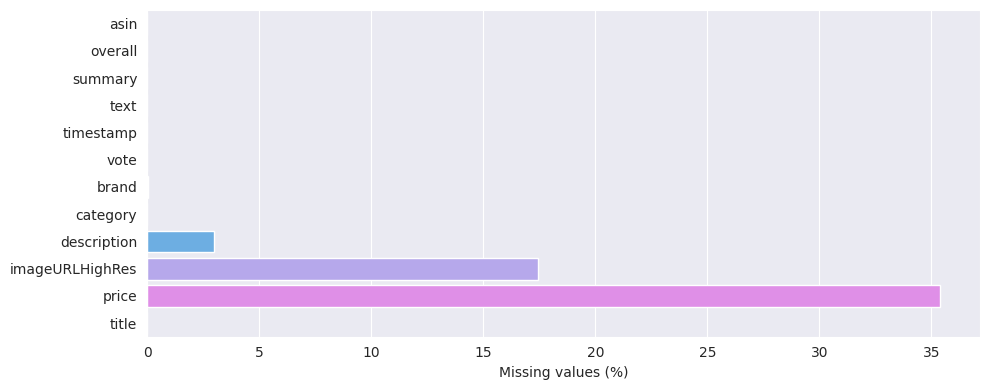
\includegraphics[width=0.95\textwidth]{images/dataset/missing_values.png}
  \caption{Percentuale dei valori mancanti per ogni attributo.}
  \label{fig:missing_values}
\end{figure}

Tramite il modello FastText \cite{joulin2016bag} sono state identificate e tenute 
solo le recensioni in lingua inglese con probabilità superiore o uguale al 95\%.

% TODO: riscrivere meglio
In input al modello è stato passato il campo \textit{text} in cui sono stati rimossi gli URL e i tag HTML e infine trasformato in minuscolo.

Il numero di recensioni rimanenti è 183,856 che corrisponde al 68\% del dataset.

% TODO: controllare cbe siano giusti data l'analisi divisa tra prodotti e reviews...

\subsection{Analisi}
Successivamente è stata effettuata un'analisi esplorativa del dataset pulito.
